\documentclass[11pt]{beamer}
\usetheme[
%%% options passed to the outer theme
    progressstyle=fixedCircCnt,   %either fixedCircCnt, movCircCnt, or corner
    rotationcw,          % change the rotation direction from counter-clockwise to clockwise
    shownavsym          % show the navigation symbols
  ]{AAUsimple}

\definecolor{darkblue}{RGB}{51,51,179}

% If you want to change the colors of the various elements in the theme, edit and uncomment the following lines
% Change the bar and sidebar colors:
\setbeamercolor{AAUsimple}{fg=gray!50 ,bg=darkblue}
\setbeamercolor{sidebar}{bg=gray!20}
\setbeamercolor{frametitle}{fg=darkblue!5,bg=darkblue}
% Change the color of the structural elements:
\setbeamercolor{structure}{fg=darkblue}
% Change the frame title text color:
%\setbeamercolor{frametitle}{fg=darkblue!20}
% Change the normal text color background:
%\setbeamercolor{normal text}{fg=black,bg=gray!10}
% ... and you can of course change a lot more - see the beamer user manual.

\usepackage[utf8]{inputenc}
\usepackage[spanish]{babel}
\usepackage[T1]{fontenc}
% Or whatever. Note that the encoding and the font should match. If T1
% does not look nice, try deleting the line with the fontenc.
\usepackage{helvet}

% colored hyperlinks
\newcommand{\chref}[2]{%
  \href{#1}{{\usebeamercolor[bg]{AAUsimple}#2}}%
}

\title{Sistema de control para estación autónoma marítima de monitoreo de ruido ambiente}

\subtitle{Presentación del Trabajo Final de Maestría}  % could also be a conference name

\date{\today}

\author{Esp. Ing. Patricio Bos }

\institute[
%  {\includegraphics[scale=0.2]{aau_segl}}\\ %insert a company, department or university logo
  Dept.\ de electrónica\\
  Facultad de Ingeniería\\
  Universidad de Buenos Aires
] % optional - is placed in the bottom of the sidebar on every slide
{% is placed on the bottom of the title page
  Maestría en Sistemas Embebidos\\
  Facultad de Ingeniería\\
  Universidad de Buenos Aires
  
  %there must be an empty line above this line - otherwise some unwanted space is added between the university and the country (I do not know why;( )
}

% specify a logo on the titlepage (you can specify additional logos an include them in 
% institute command below
\pgfdeclareimage[height=1.5cm]{titlepagelogo}{imagenes/logo_facu_circle} % placed on the title page
%\pgfdeclareimage[height=1.5cm]{titlepagelogo2}{AAUgraphics/aau_logo_new} % placed on the title page
\titlegraphic{% is placed on the bottom of the title page
  \pgfuseimage{titlepagelogo}
%  \hspace{1cm}\pgfuseimage{titlepagelogo2}
}

\definecolor{darkblue}{RGB}{51,51,179}
\setbeamercolor{bgcolor}{fg=white,bg=darkblue}

\setbeamertemplate{navigation symbols}{}
\beamerdefaultoverlayspecification{<+->}

\AtBeginSection[]
{
 \begin{frame}<beamer>
 \frametitle{\textbf{\LARGE{Agenda}}}
 \fontsize{18pt}{18}\selectfont
 \tableofcontents[currentsection]
 \end{frame}
}

\begin{document}

\begin{frame}[plain,noframenumbering]
	\begin{center}
	\vspace{5px}	
	\Large\textbf{Maestría en Sistemas Embebidos - FIUBA}\\
	\vspace{10px}
	\large\textbf{Presentación de Trabajo Final}\\
	\vspace{5px}
  \begin{beamercolorbox}[center,sep=1.125ex,dp=1.125ex,ht=18ex, wd=\paperwidth]{bgcolor}
	  \huge\textbf{Sistema de control para estación autónoma marítima de monitoreo de ruido ambiente}\\
    	\vspace{5px}
	  \Large\textbf{Esp. Ing. Patricio Bos}\\
  \end{beamercolorbox}
%	\vspace{10px}
	\vfill
	\begin{minipage}[t]{0.47\textwidth}
		\begin{flushleft} \large
			\textbf{Director:}\\
			Dr. Ing Ariel Lutenberg
		\end{flushleft}
	\end{minipage}
	\hfill
	\begin{minipage}[t]{0.47\textwidth}
		\begin{flushright} \large
			\textbf{Jurados:} \\
			Dr. Ing. Pablo Gómez \\
			Ing. Juan Manuel Cruz\\
			Mg. Lic Igor Prario\\
		\end{flushright}
	\end{minipage}
%	\vfill
%	\begin{figure}[H]
%		
\includegraphics[width=2cm]{./imagenes/logo_facu_circle}
%	\end{figure}	
%	\vspace{5px}
	\end{center}
\end{frame}

% TOC
\begin{frame}{\textbf{\LARGE{Agenda}}}
\fontsize{18pt}{18}\selectfont
\tableofcontents
\end{frame}
%%%%%%%%%%%%%%%%

\section{Motivación}

\begin{frame}{\textbf{\LARGE{Motivación}}}
\fontsize{18pt}{18}\selectfont
	\vspace{-.7cm}
	\centering
	\begin{itemize}
	\item ¿Por qué acústica submarina?
	\vspace{15px}
	\item ¿Qué es el nivel de ruido?
	\vspace{15px}
	\item ¿Por qué interesa medirlo?
	\vspace{15px}	
	\item ¿Qué disciplinas lo necesitan?
%	\item 
	\end{itemize}
\end{frame}

\begin{frame}{\textbf{\LARGE{Antecendentes}}}
	\vspace{-.6cm}
		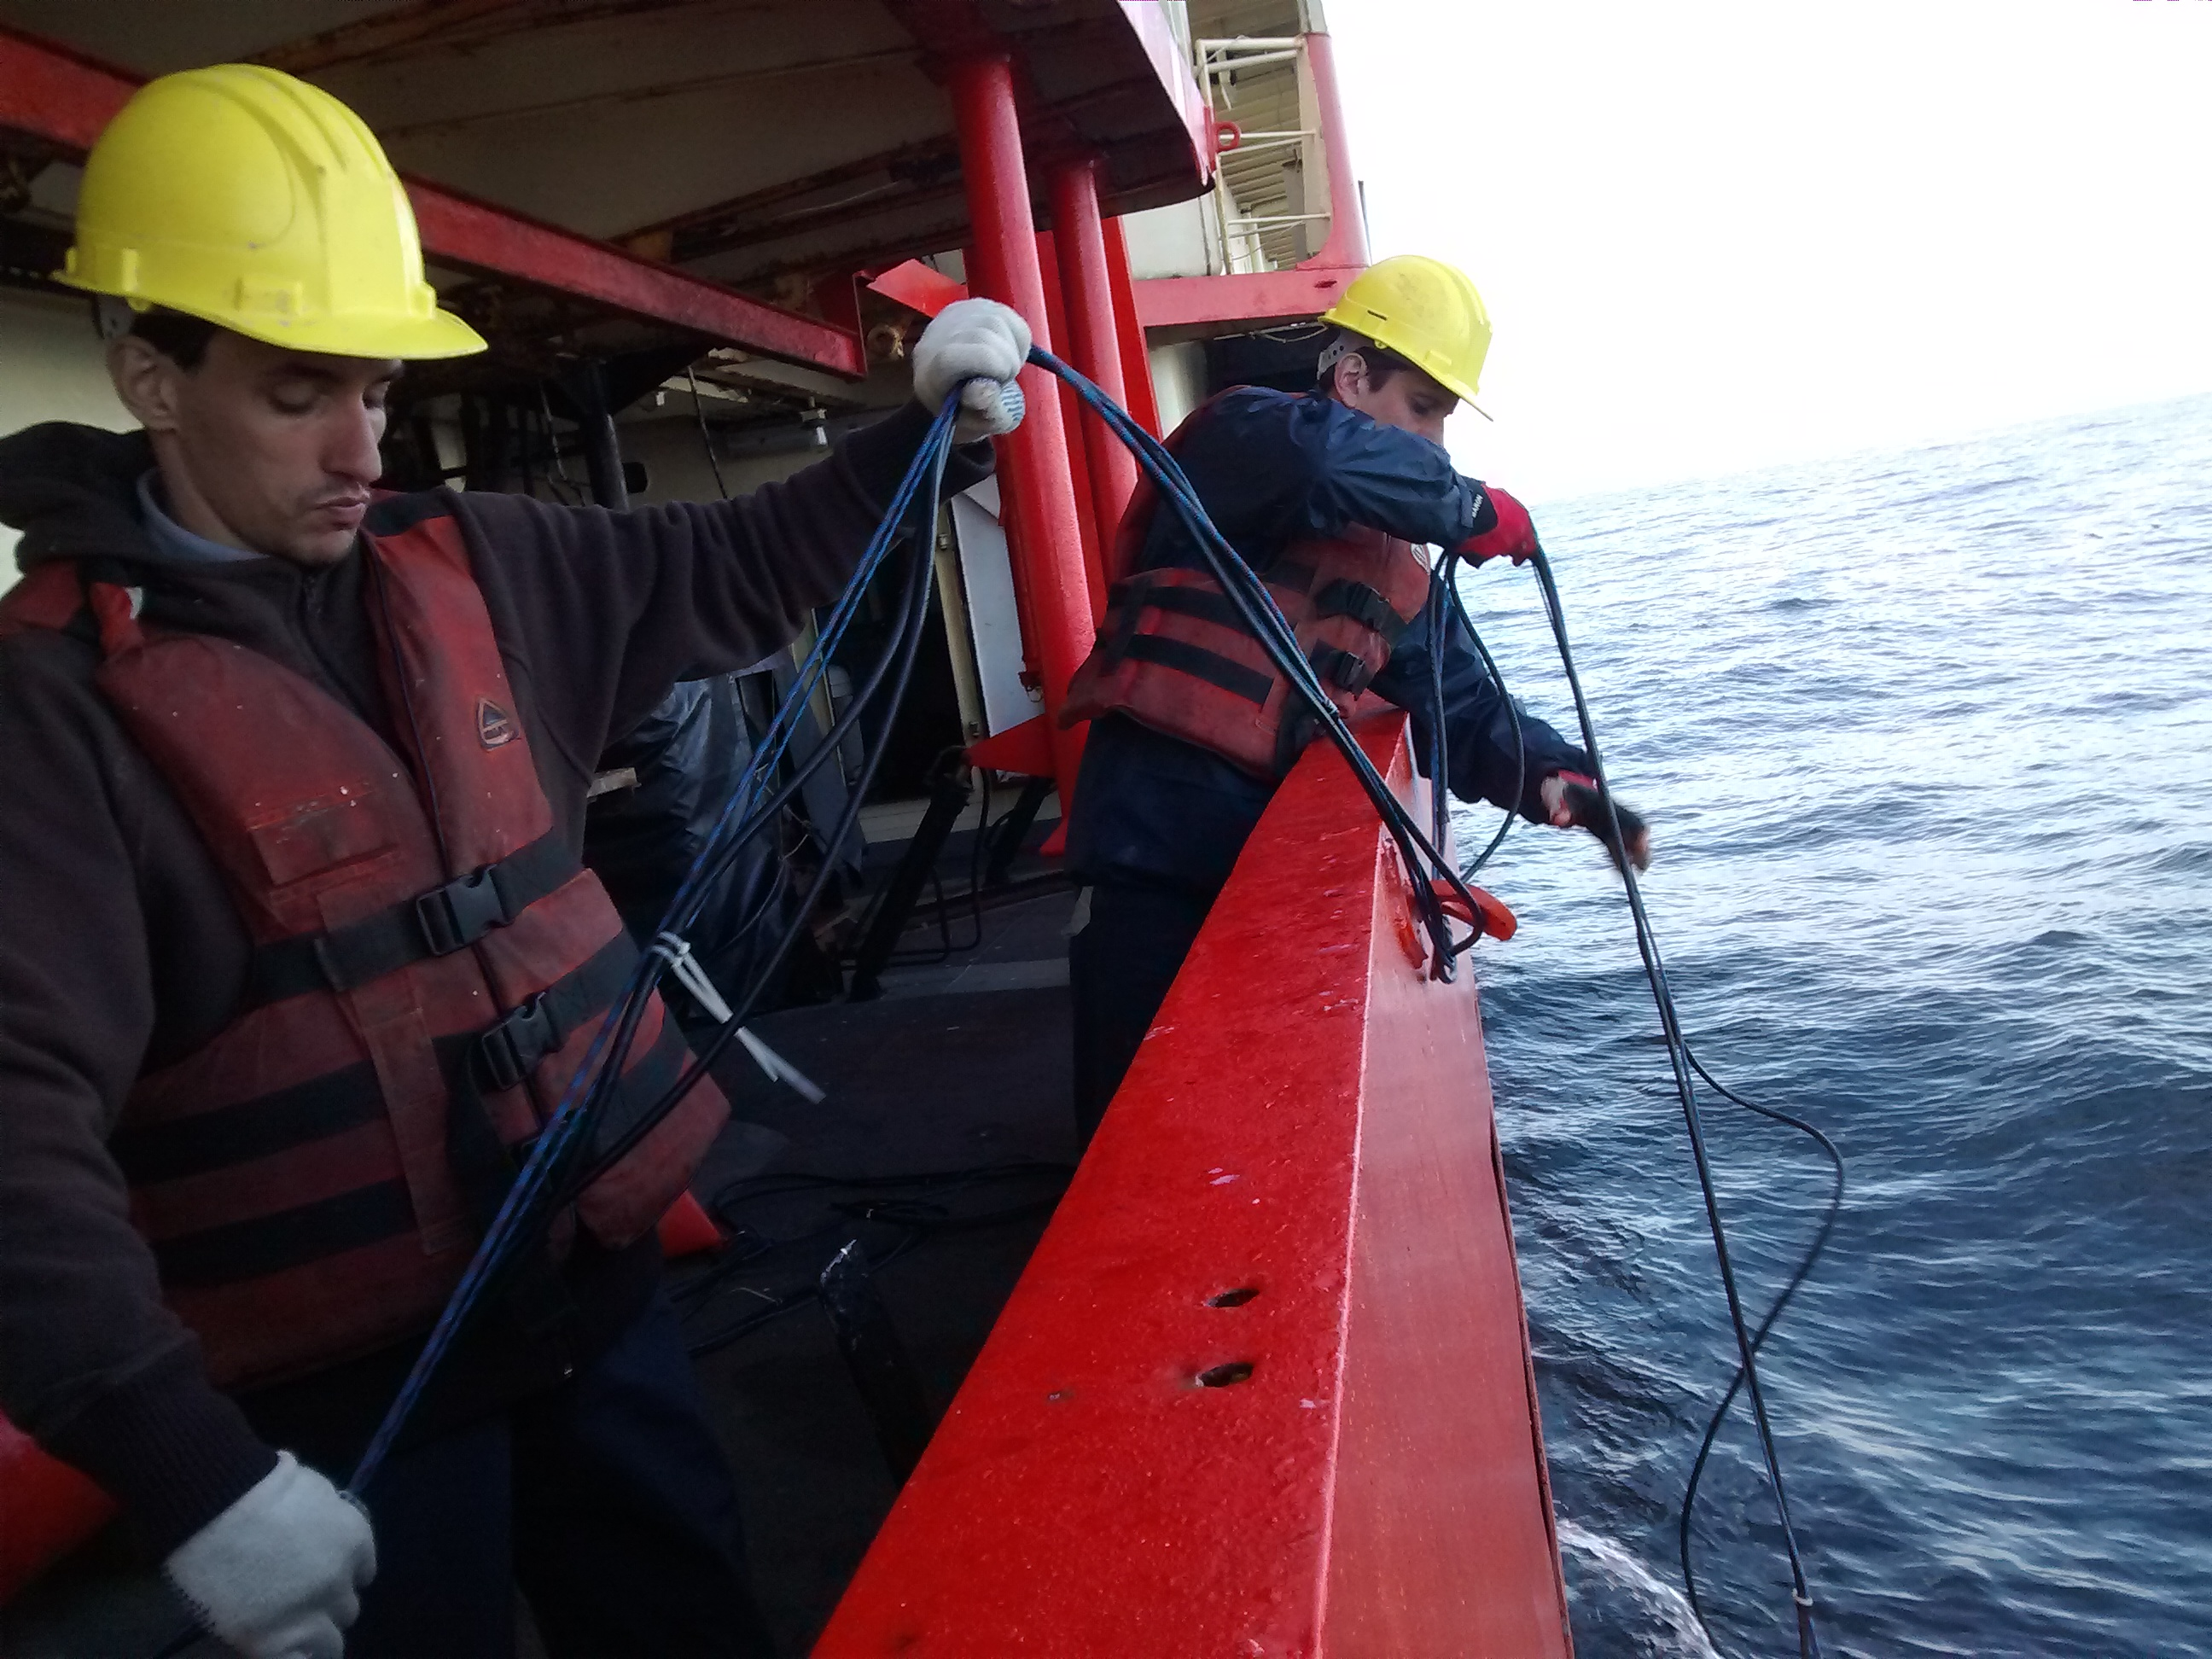
\includegraphics[width=.9\textwidth]{./imagenes/antecedentes.jpg}
\end{frame}

\section{Planificación}

\begin{frame}{\textbf{\LARGE{Diagrama en bloques}}}
	\vspace{-.6cm}
		\includegraphics[width=\textwidth]<1>{./imagenes/Diagrama_en_Bloques.pdf}
		\includegraphics[width=\textwidth]<2>{./imagenes/Diagrama_en_Bloques_recorte.pdf}
\end{frame}

\begin{frame}{\textbf{\LARGE{Planificación en etapas}}}
	\vspace{-.7cm}
	\begin{figure}[H]
		{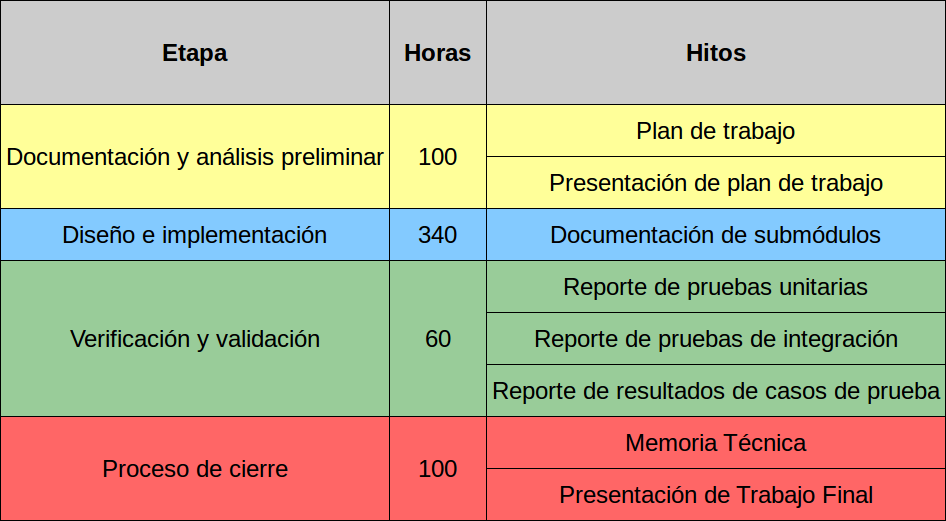
\includegraphics[width=\textwidth]{./imagenes/planificacion.png}}
	\end{figure}	
\end{frame}

\begin{frame}{\textbf{\LARGE{Desglose de tareas en AoN}}}
	\vspace{-.7cm}
	\begin{figure}[H]
		{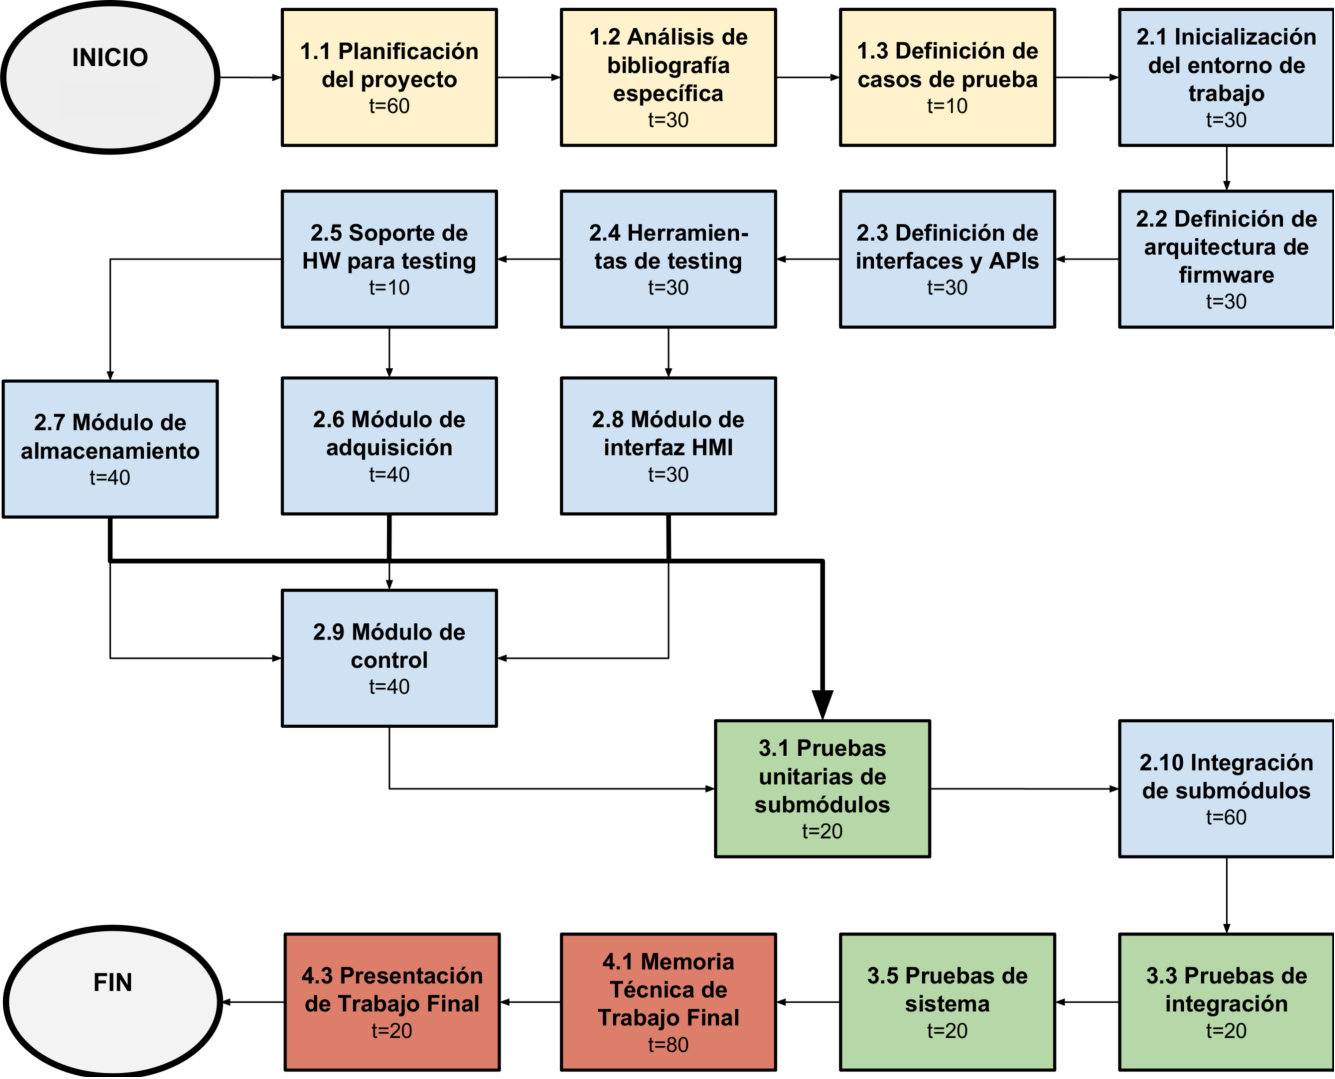
\includegraphics[height=.8\textheight]{./imagenes/AoN.pdf}}
	\end{figure}	
\end{frame}


\section{Metodología}

\begin{frame}{\textbf{\LARGE{Modelo de ramas}}}
	\vspace{-.7cm}
	\begin{figure}[H]
		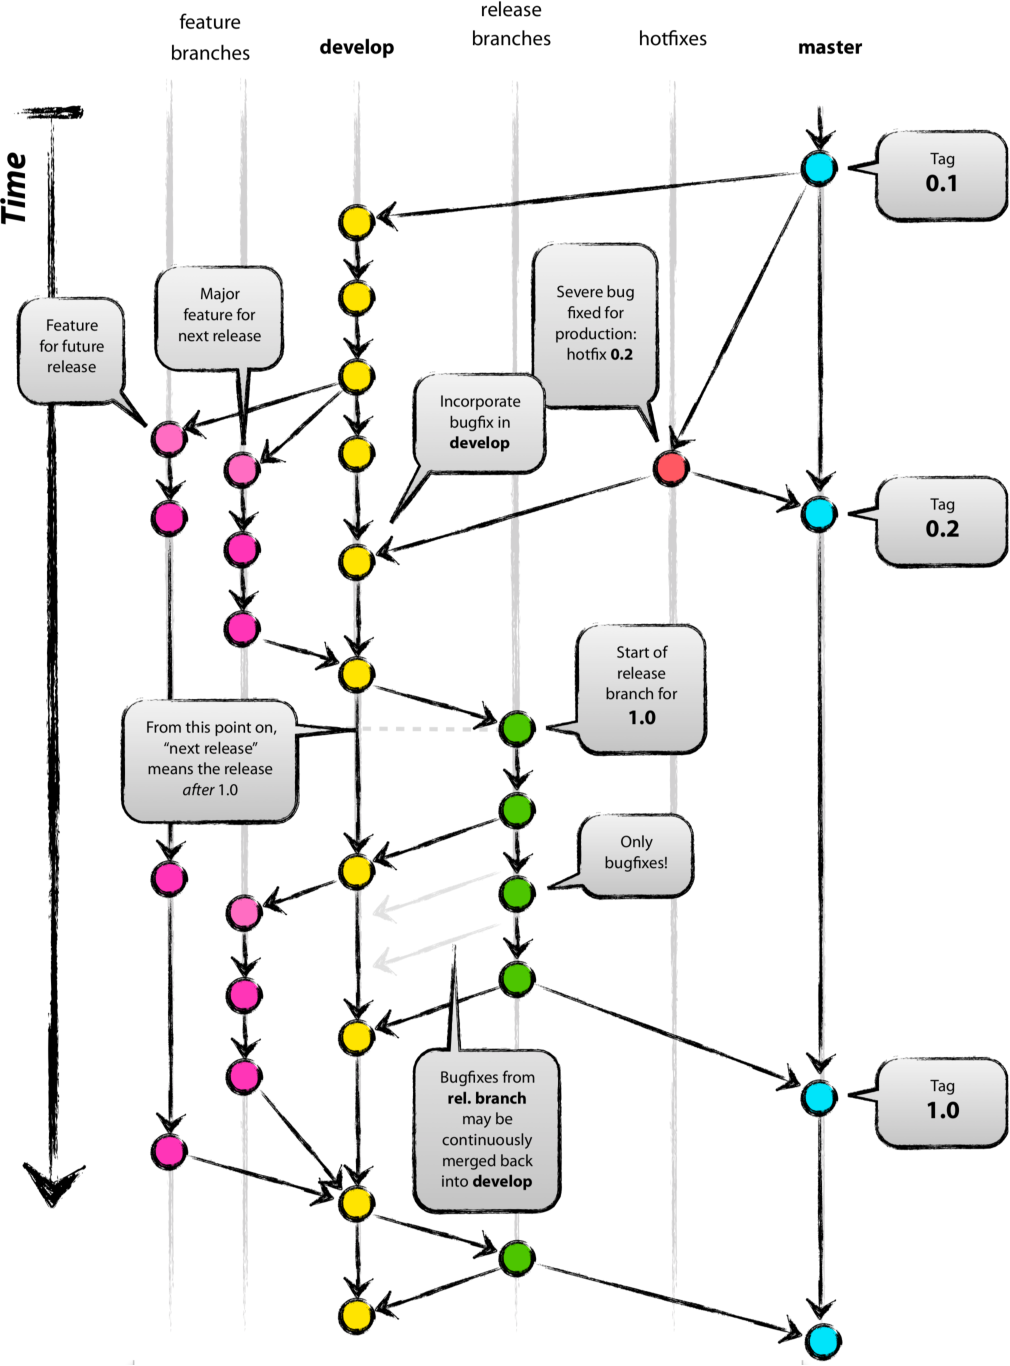
\includegraphics[height=.8\textheight]{./imagenes/Git-branching-model.pdf}
	\end{figure}	
\end{frame}


\begin{frame}{\textbf{\LARGE{Inter Process Communications}}}
	\vspace{-.7cm}
	\begin{figure}[H]
		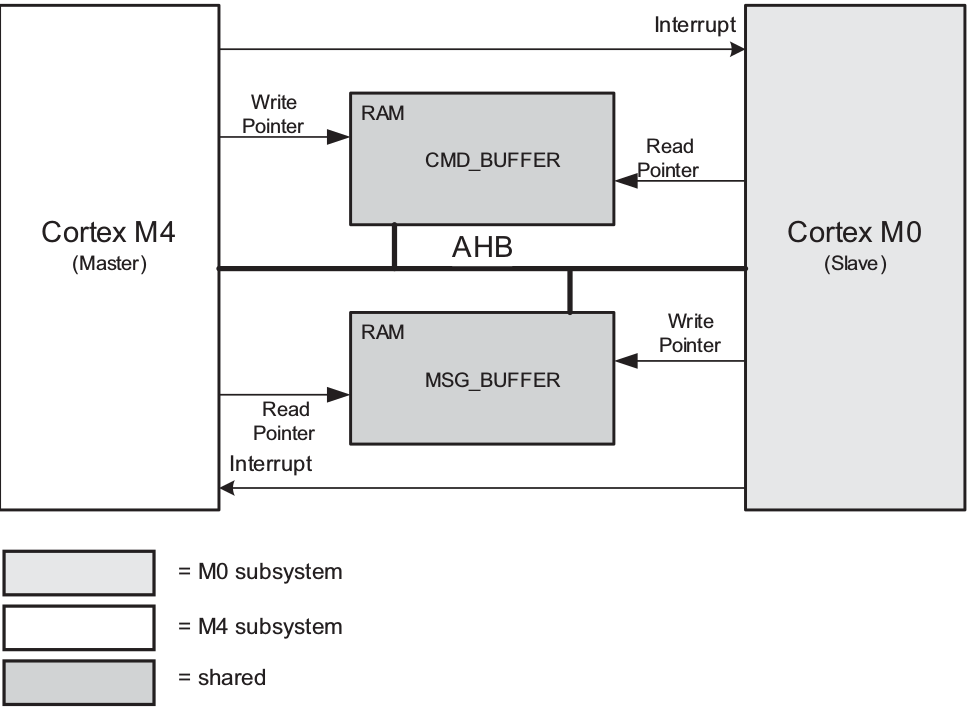
\includegraphics[height=.8\textheight]{./imagenes/IPC.png}
	\end{figure}	
\end{frame}

\section{Implementación}

\begin{frame}{\textbf{\LARGE{Modelo de capas}}}
	\vspace{-.7cm}
	\begin{figure}[H]
		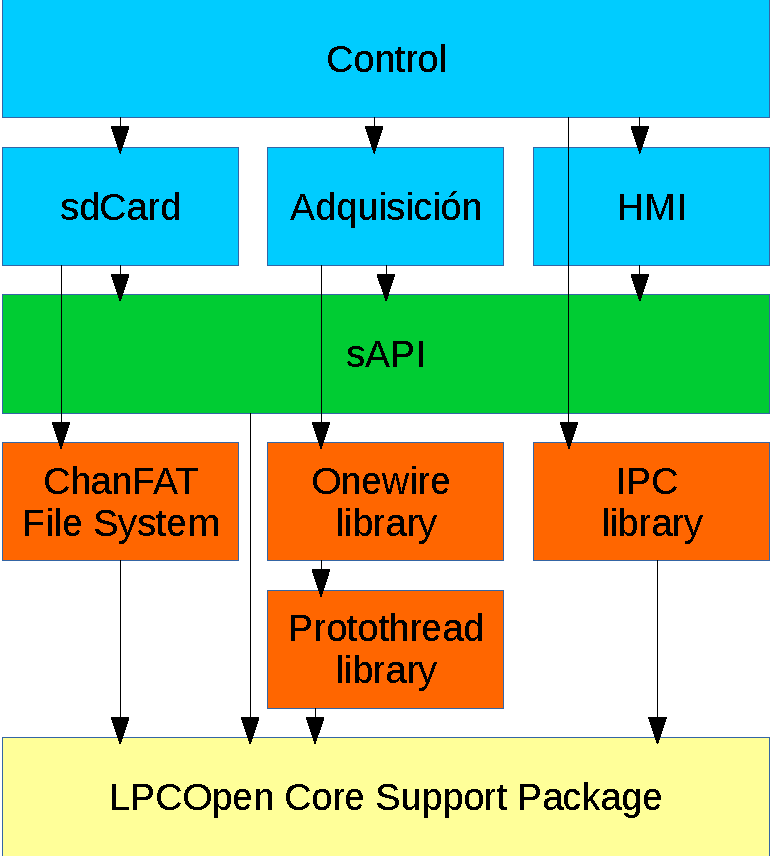
\includegraphics[height=.8\textheight]{./imagenes/capas.pdf}
	\end{figure}	
\end{frame}

\begin{frame}{\textbf{\LARGE{Modelo de ramas}}}
	\vspace{-.7cm}
	\begin{figure}[H]
		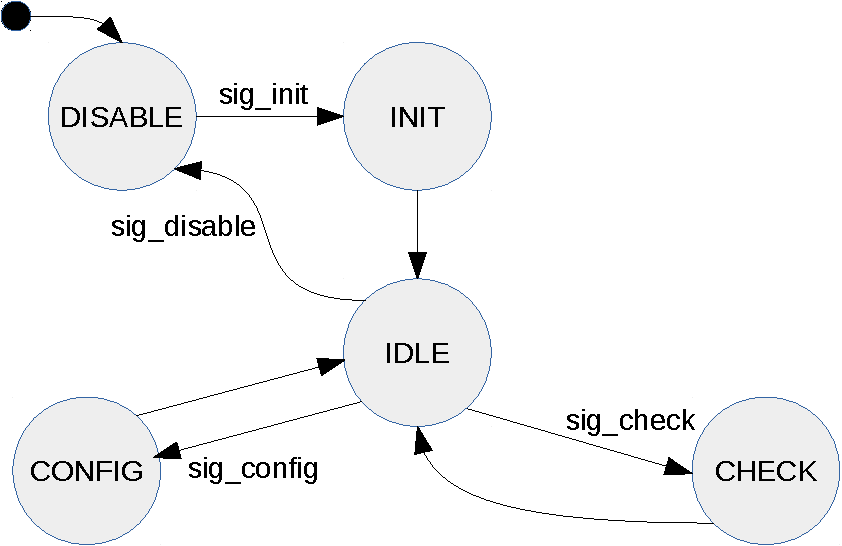
\includegraphics[height=.8\textheight]{./imagenes/MEF_generica.pdf}
	\end{figure}	
\end{frame}

\section{Testing}

\begin{frame}{\textbf{\LARGE{Modelo de ramas}}}
	\vspace{-.7cm}
	\begin{figure}[H]
		{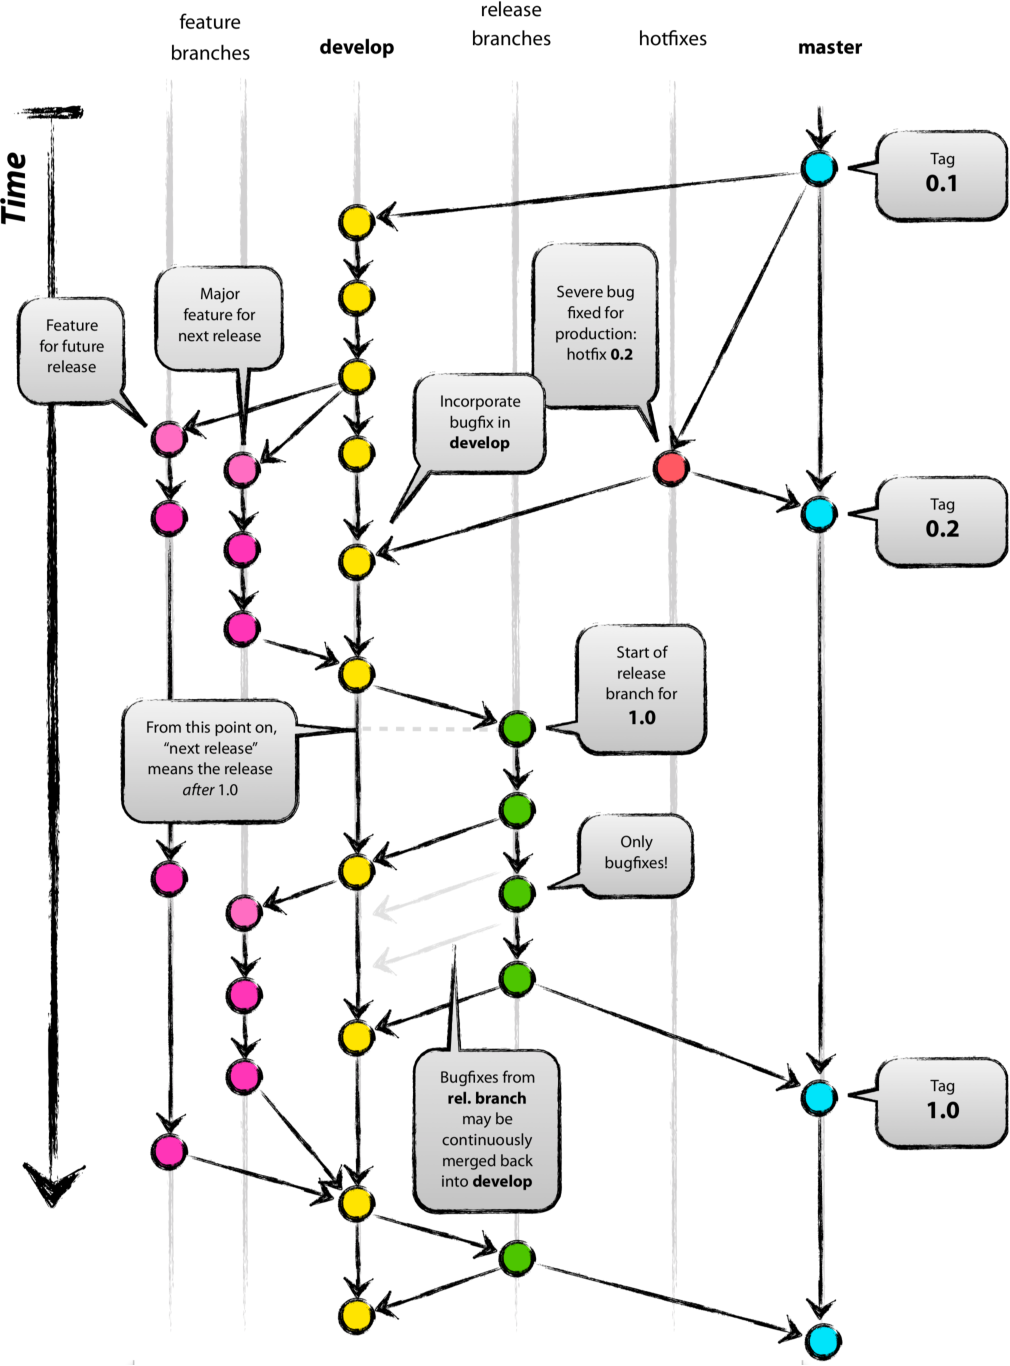
\includegraphics[height=.8\textheight]{./imagenes/Git-branching-model.pdf}}
	\end{figure}	
\end{frame}

\section{Demo}

\begin{frame}{\textbf{\LARGE{Modelo de ramas}}}
	\vspace{-.7cm}
	\begin{figure}[H]
		{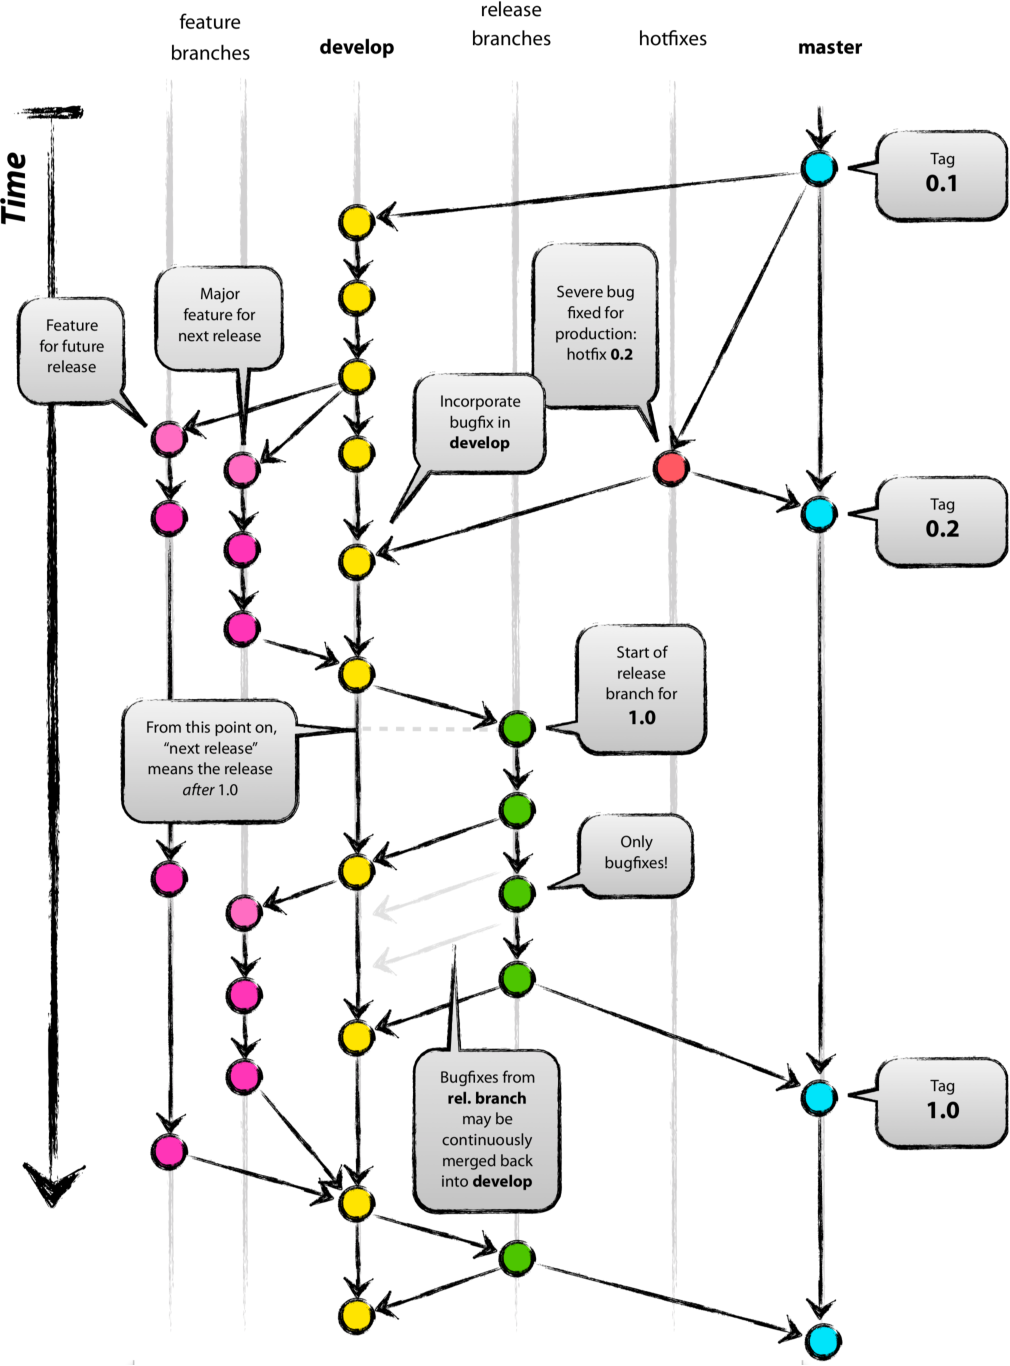
\includegraphics[height=.8\textheight]{./imagenes/Git-branching-model.pdf}}
	\end{figure}	
\end{frame}

\section{Conclusiones}



\begin{frame}{\textbf{\LARGE{¿Sobre qué hace falta alertar?}}}
\fontsize{18pt}{18}\selectfont

\end{frame}

\begin{frame}{\textbf{\LARGE{Tecnologías utilizadas}}}
\fontsize{18pt}{18}\selectfont
\end{frame}

\end{document}
